% !TEX root = calculus.tex


\chapter{DIFFERENTIAL EQUATIONS}
\label{diff-eqns}

\athr You are, certainly, familiar with various types of equations: algebraic, logarithmic, exponential, trigonometric. They have a common feature: by solving these equations one arrives at \emph{numbers} (these are the so-called ``roots'' of equations). Now we are going to deal with a very different type of equations, namely, \emph{equations whose solutions are functions}. Among the equations subsumed into this class are the so-called \emph{differential equations}.

Consider a function $f (x)$. We denote its first derivative (the first-order derivative) by $f' (x)$, its second derivative by $f''(x)$, its third derivative by $f''' (x)$, and so on.

\begin{mytheo}{Definition:}
A differential equation is an equality relating $x, \, f (x), \, f' (x), \, f'' (x)$, etc. A solution of a differential equation is a junction $f (x)$.
\end{mytheo}
\rdr So far you have never mentioned the concepts of second derivative or third derivative.

\athr True, and this is what we are going to do right now.

\rdr It is readily apparent that since a derivative $f (x)$ is a \emph{function}, it can be differentiated, thus yielding a \emph{derivative of the derivative}; I guess, this must be the second derivative of the original function $f (x)$.

\athr By differentiating the function $f (x)$ $n$ times o(of course, if this can be done with the given function), we obtain a derivative of the $n$th order (in other words, ``the $n$th derivative''). Thus, the third derivative of $f (x)$ is obviously,
\begin{equation*}%
f'''(x) = \ddx \left[ \ddx \left( \ddx f (x) \right) \right]
\end{equation*}
 Note that we are, in fact, familiar with the second derivative. As the function $f (x)$ is the first derivative of an anti-derivative $F (x) [f (x)= F' (x)]$, the function $f'' (x)$ can be considered as the second derivative of the antiderivative $F (x)$:
\begin{equation*}%
 f' (x) = F" (x)
\end{equation*}
 
 \rdr We know that the derivative of $f (x)$ (to be exact, its \emph{first} derivative) is the rate of change of this function. Its magnitude is reflected in the slope of the graph of the function $f (x)$ at each point and is measured as the tangent of the angle between the tangent line to the graph and the abscissa axis. Could anything of this type be said about the \emph{second} derivative of $f (x)$?
 
\athr Evidently, the second derivative of $f (x)$ characterizes the rate at which \emph{the rate of change of the function changes with $x$}, so that it is a finer characteristic of the behaviour of the initial function. Look at \fig{fig-53}. What is the difference between functions $f_{1}$ and $f_{2}$ at point $x = x_{0}$?


\begin{figure}[!ht]%[13]{r}{0.5\textwidth}
\centering
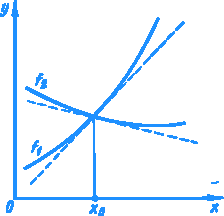
\includegraphics[width=.6\textwidth]{figures/fig-53.pdf} 
\caption{Examining behavior of functions and their derivatives at a point.}
\label{fig-53}
\end{figure}


\rdr They have different first derivatives. I can write:
\begin{equation*}%
f_{1} (x_{0}) = f_{2} (x_{0}), \quad	f_{1}' (x_{0}) \neq f_{2}' (x_{0})
\end{equation*}
\athr To complete the picture, note that at the point in question the derivatives differ both in magnitude (the figure clearly shows that $| f_{2}' (x_{0}| < |f_{1}' (x_{0})|$ and in sign: $ f_{1}' (x_{0}) >0, \,\, f_{2}' (x_{0}) < 0$. We say, therefore, that the function $f_{1}$ \emph{increases} (and rather rapidly) at point $x = x_{0}$, while the function $f_{2}$ \emph{decreases} (and comparatively slowly).

Now turn to \fig{fig-54}. We observe that not only the values of the functions $f_{1}$ and $f_{2}$ but also the values of their first derivatives coincide at point  $x = x_{0}$:
\begin{equation*}%
f_{1} (x_{0}) = f_{2} (x_{0}), \quad	f_{1}' (x_{0}) = f_{2}' (x_{0})
\end{equation*}
However, the graph shows a difference in the behaviour of the functions $f_{1}$ and $f_{2}$ in the vicinity of $ x_{0}$. Try to describe this difference.

\begin{figure}[!ht]%[13]{r}{0.5\textwidth}
\centering
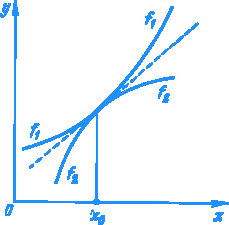
\includegraphics[width=.6\textwidth]{figures/fig-54.pdf} 
\caption{Examining behavior of functions and their derivatives at a point.}
\label{fig-54}
\end{figure}

\rdr In the vicinity of $ x_{0}$ the graph of the function $f_{1}$ is convex downward, while that of the function $f_{2}$ is convex upward. Besides, the curvature is greater for the function $f_{2}$ than for $f_{1}$.

\athr These are precisely the finer features of the behaviour of $f_{1}$ close to $x = x_{0}$, and they can be identified by finding the value of the second derivative at $x_{0}$ (by calculating the value of $f'' (x_{0})$). In the case shown in \fig{fig-54} we have
\begin{equation*}%
f_{1}'' (x_{0}) \neq f_{2}'' (x_{0})
\end{equation*}
You will immediately see that $f_{1}'' (x_{0}) > 0$ and $ f_{1}'' (x_{0}) < 0$. Indeed, the slope of $f_{1}$ at $x_{0}$ steadily increases; hence, the slope of $f_{1}'$ is \emph{positive}. On the contrary, the slope of $f_{2}$ at $x_{0}$ steadily decreases; hence, the slope of  $f_{2}'$ is \emph{negative}. It is quite obvious (see the figure) that
\begin{equation*}%
\left| f_{1}'' (x_{0}) \right| < \left|f_{2}'' (x_{0}) \right|
\end{equation*}

\rdr In all likelihood, the third derivative of $f (x)$, i.e, $f''' (x_{0})$, is a still finer 
characteristic of the behaviour of  $f(x)$ at $x= x_{0}$. Am I right?

\athr Precisely. Unfortunately, it is virtually impossible to illustrate this simply enough on a graph of the function $f (x)$.

I think that it is enough for a discussion of derivatives of different orders; let us move on to \emph{differential equations}. Note, first of all, that an equation of the type
\begin{equation}%
f' (x) = \varphi \, (x)
\label{diff-eq-1}
% eq 1 of 13
\end{equation}
where $\varphi \, (x)$ is a given function, can be considered as the simplest particular case in the theory of differential equations; its solution is obtained by a straightforward integration.

Two simple (and, incidentally, very frequently encountered) types of differential equations are
\begin{equation}%
\boxed{f' (x) = p \, f(x)}
\label{exp-growth}
% eq 2 of 13
\end{equation}
\begin{equation}%
\boxed{''(x)= - q\, f(x) \quad (q>0)}
\label{harmonic-osc}
% eq 3 of 13
\end{equation}
where $p$ and $q$ are constants.

Equation \eqref{exp-growth} is called the \emph{differential equation of exponential growth (decay)}, and equation \eqref{harmonic-osc} is the differential equation of harmonic oscillations.

Let us look at these equations more closely. We begin with the differential equation of exponential growth (decay). What conclusions can be drawn from the form of this equation?

\rdr The form of equation \eqref{exp-growth} shows that the rate of change of the function $f (x)$ coincides with the value of the function, to within a constant factor $p$; at each point $x$, In other words, the function $f (x)$ and its first derivative $f' (x)$ coincide, to within the mentioned factor, at each point $x$.

\athr Please, recall \hyperref[differentiation]{Dialogue Ten} and tell me what functions could serve as solutions of this equation. What are the functions for which the derivative coincides with the function itself? In other words, what functions are transformed by differentiation into themselves?

\rdr This property is typical of the exponential function $a^{x}$ for $a = e$. It is called the exponential curve and is often denoted by $\exp \, (x)$. We have found in \hyperref[differentiation]{Dialogue Ten}  that
\begin{equation*}%
\ddx \exp (x) =	\exp (x)
\end{equation*}
\athr Correct. This means that the function $f (x) = \exp \, (px)$ must be taken as a solution of the equation $f' (x) = p \, f (x)$. Indeed,
\begin{align*}%
\ddx \exp \, (px) & = \left( \dfrac{d}{dy} \exp \, (y) \right) \ddx (px) \\
& = p \exp \, (y) =p \exp \, (px)
\end{align*}
For this reason equation \eqref{exp-growth} is called the differential equation of \emph{exponential} growth (decay). Obviously, we have growth if $p > 0$, and decay if $p <0$.

\rdr Apparently, any function
\begin{equation*}%
 f (x) = C \exp \, (px)
\end{equation*}
where $C$ is an arbitrary constant factor, is a solution of this equation, because the constant $C$ is factored out of the derivative.

\athr You are absolutely right.
\begin{mytheo}{}
A solution of a differential equation $f' (x) = p \, f (x)$ is a family of functions
\begin{equation*}%
f(x)= C \exp \, (px)
\end{equation*}
with an arbitrary constant factor $C$ (usually referred to as the integration constant).
\end{mytheo}

Some of functions $C \exp \, (px)$ are plotted in \fig{fig-55} (we have specified $p > 0$).

\begin{figure}[!ht]%[13]{r}{0.5\textwidth}
\centering
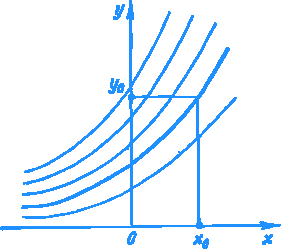
\includegraphics[width=.6\textwidth]{figures/fig-55.pdf} 
\caption{Graphs of some of functions $C \exp \, (px)$.}
\label{fig-55}
\end{figure}


The formula $f (x) = C \exp \, (px)$, describing the whole family of functions, is called the \emph{general solution} of a given differential equation. By fixing (i.e. specifying) a value of $C$, one selects (singles out) a \emph{particular solution} from the general solution.

\rdr How can it be done?

\athr Oh, this is elementary. It is sufficient to prescribe a specific value to the function $f (x)$ at a certain point. For example, let us prescribe
\begin{equation*}%
f (x_{0}) = y_{0}
\end{equation*}
In this case we are interested in a single curve among the curves of the whole family (see \fig{fig-55}; the selected curve is shown by a thicker solid line). This curve is a graph of the function $C \exp \, (px)$ for which $C \exp \, (p x_{0}) = y_{0}$, and, therefore, $C = y_{0} \exp (-px_{0})$. Consequently, the particular solution we are seeking for has the form
\begin{equation}%
 f(x) = y_{0} \exp \, [p(x- x_{0})]
 \label{exp-soln}
 % eq 4 of 13
\end{equation}
\rdr We thus obtain that in order to find a specific (particular) solution of the differential equation $f' (x) = p f (x)$, it is necessary to supplement the equation with an additional condition: $f (x_{0}) = y_{0}$.

\athr Precisely. This condition is called the \emph{initial condition.}

Let us turn now to differential equation \eqref{harmonic-osc}:
 \begin{equation*}%
f''(x) = -q \, f(x) \quad (q>0)
\end{equation*}

\rdr In this case the value of the function $f (x)$ coincides at each point not with the rate of change of the function but with the rate of change of its rate of change, with the sign reversed.

\athr In other words, the function $f (x)$ is equal, to within a constant factor, to its second derivative $f'' (x)$. Recall what functions have this property.

\rdr I guess that the solutions of equation \eqref{harmonic-osc} are functions $\sin x$ or $\cos x$.

\athr To be	precise: $\sin \, (\sqrt{q} x)$	or	$\cos \, (\sqrt{q}x)$. Indeed,
\begin{align*}%
\ddx \left( \ddx \sin (\sqrt{q}x) \right) & = \sqrt{q} \ddx \cos (\sqrt{q}x) = - q \sin (\sqrt{q} x) 
\end{align*}
or
\begin{align*}%
\ddx \left( \ddx \cos (\sqrt{q}x) \right) & = - \sqrt{q} \ddx \sin (\sqrt{q}x) = - q \cos (\sqrt{q} x) 
\end{align*}
This is why the equation in question is called the differential equation of \emph{harmonic oscillations}.

It is easily seen that the general solution of equation \eqref{harmonic-osc} can be written in the form
\begin{equation}%
f(x)= C_{1} \sin (\sqrt{q} x) + C_{2} \cos (\sqrt{q}x)
 \label{harmonic-soln}
 % eq 5 of 13
\end{equation}
where $C_{1}$ and $C_{2}$ are arbitrary constants (integration constants). Indeed, 
\begin{align*}%
f'(x) &= \sqrt{q} \, C_{1} \cos (\sqrt{q} x) + - \sqrt{q} \, C_{2} \sin (\sqrt{q}x) \\
f''(x) &= -[q  \, C_{1} \sin (\sqrt{q} x) + \, C_{2} \sin (\sqrt{q}x) ]\\
& = -q \, f(x)
\end{align*}

\rdr But this gives us \emph{two} integration constants instead of one, as in the preceding case.

\athr Yes, and the reason is that differential equation \eqref{harmonic-osc} contains the \emph{second} derivative. Hence, it is necessary to integrate \emph{twice} in order to obtain the function $f (x)$. And we know that each integration leads to a family of anti-derivatives, that is, generates an integration constant. In the general case, the number of integration constants in the general solution of a specific differential equation equals the \emph{maximum} order of derivative in this equation. The general solution of equation \eqref{exp-growth} has a single integration constant because it contains only the first derivative of the sought function and does not involve derivatives of higher order. The general solution of equation \eqref{harmonic-osc} has two integration constants because the equation contains the second-order derivative of the sought function and no derivatives of higher order.

\rdr And how do we write the initial condition for equation \eqref{harmonic-osc}?

\athr One has to prescribe at a point $x = x_{0}$ a value not only to the sought function but also to its first derivative. In this case the initial conditions are written as follows:
\begin{equation}%
f(x_{0})= f_{0} \quad f'(x_{0})= f_{0}'
\label{initial-condn}
 % eq 6 of 13
\end{equation}

\rdr And if a differential equation involved the third derivative, and the general solution contained, as a result, not two but three integration constants? 

\athr In this case the initial conditions would prescribe values to the required function, its first derivative, and its second derivative at a point $x = x_{0}$:
\begin{equation*}%
f(x_{0})= f_{0} \quad f'(x_{0})= f_{0}' \quad f''(x_{0})= f_{0}'' 
\end{equation*}
But let us return to the general solution of equation \eqref{harmonic-osc}. It is usually written not in form \eqref{harmonic-soln} but in a somewhat different form. Namely, either
\begin{equation}%
f(x)= A \, \sin (\sqrt{q} x + \alpha)
 \label{harm-soln2}
 % eq 7 of 13
\end{equation}
or
\begin{equation}%
f(x)= A \, \cos (\sqrt{q} x + \beta)
\tag{\ref{harm-soln2}a}
\label{harm-soln3}
 % eq 7a of 13
\end{equation}

Formula \eqref{harm-soln3} is obtained from \eqref{harm-soln2} if we set $\alpha = \beta + \dfrac{\pi}{2}$.

In what follows we shall use notation \eqref{harm-soln2}. In this form the role of the integration constants $C_{1}$ and $C_{2}$ in general solution \eqref{harmonic-soln} is played by constants $A$ and $\alpha$. Formula \eqref{harmonic-soln} is easily transformed by trigonometry to \eqref{harm-soln2}, by using the formula for the sine of a sum. Indeed,
 \begin{equation*}%
A \sin (\sqrt{q}x + \alpha) = A \sin (\sqrt{q}x) \cos \alpha + A \cos (\sqrt{q}x) \sin \alpha
\end{equation*}
so that
 \begin{equation*}%
C_{1} = A \cos \alpha,	\quad C_{2} = A \sin \alpha 
\end{equation*}
Now try to obtain from general solution \eqref{harm-soln2} a particular solution satisfying initial conditions \eqref{initial-condn}.

\rdr We shall obtain it by expressing the constants
$A$ and $a$ via $f_{0}$ and $f_{0}'$ the first derivative of $f (x)$:

Equality \eqref{harm-soln2} yields an expression for 
 \begin{equation*}%
f'(x) = A \sqrt{q} \cos (\sqrt{q}x + \alpha )
\end{equation*}
In this case initial conditions \eqref{initial-condn} take the form 
\begin{equation}%
\begin{split}
\sin (\sqrt{q} x_{0} + \alpha) & = \frac{f_{0}}{A} \\
\cos (\sqrt{q} x_{0} + \alpha) & = \frac{f_{0}'}{A \sqrt{q}} 
\end{split}
\label{intial-condn2}
%eq 8 of 13
\end{equation}
System \eqref{intial-condn2} must be solved for the unknown constants $A$ and $\alpha$. Squaring both equations of the system and summing them up, we obtain (taking into account that $\sin^{2} \nu + \cos^{2} \nu = 1$)
 \begin{equation*}%
\left( \dfrac{f_{0}'}{A} \right)^{2} + \left( \frac{f_{0}'}{A \sqrt{q}}\right)^{2} = 1
\end{equation*}
This yields
\begin{equation}%
A  = \sqrt{f_{0}^{2} + \left( \dfrac{f^{2}_{0}\prime}{\sqrt{q}} \right)}
 \label{harm-soln3}
 % eq 9 of 13
\end{equation}
Dividing the first equation of system \eqref{intial-condn2} by the second,
we obtain 
\begin{equation}%
\tan (\sqrt{q} x_{0} + \alpha) = \dfrac{f_{0}}{f_{0}\prime} \sqrt{q}
 \label{harm-soln4}
 % eq 10 of 13
\end{equation}


From \eqref{harm-soln4} we can find constant $\alpha$.

The constants $A$ and $\alpha$, expressed in terms of $f_{0 }$ and $f_{0}\prime$ must be substituted into \eqref{harm-soln2}; the result is the particular solution satisfying initial conditions \eqref{initial-condn}.

\athr Assume that initial conditions \eqref{initial-condn} are 
\begin{equation}%
f(0)= 0, \,\,\, f\prime(0)= f_{0}'
\label{intial-condn3}
% eq 11 of 13
\end{equation}

\rdr In this case formulas \eqref{harm-soln3} and \eqref{harm-soln4} yield
\begin{equation}%
A = \dfrac{f_{0}\prime}{\sqrt{q}}
\label{harm-soln5}
% eq 12 of 13
\end{equation}

If $\tan \alpha =0$, then $\alpha= \pi n$, where $n= 0, \pm 1, \pm 2$, And since, first,	
\begin{equation*}%
\sin 	(\sqrt{q}x	+ \alpha)	=	\sin 	(\sqrt{q} x)	\cos \alpha	 + \cos (\sqrt{q}x) \sin \alpha	
\end{equation*}
and, second, in  this particular case $\sin \alpha = 0$ and $\cos \alpha =	\pm 1$, we conclude that either
\begin{equation*}%
f(x) = \dfrac{f_{0}\prime}{\sqrt{q}} \sin (\sqrt{q} x)	
\end{equation*}
or 
\begin{equation*}%
f(x) = - \dfrac{f_{0}\prime}{\sqrt{q}} \sin (\sqrt{q} x)	
\end{equation*}

\athr The second variant is unacceptable because it violates the condition $f\prime (0) =f_{0}'$.

\rdr Hence, the required particular solution is 
\begin{equation}%
f(x) = \dfrac{f_{0}\prime}{\sqrt{q}} \sin (\sqrt{q} x)	
\label{harm-soln6}
% eq 13 of 13
\end{equation}

\athr Very good. Now consider the initial conditions
in the form
\begin{equation}%
f(0)= f_{0}, \,\,\, f\prime(0)= 0
\label{intial-condn4}
% eq 14 of 13
\end{equation}

\rdr Formula \eqref{harm-soln3} yields $A = f_{0}$. However, formula \eqref{harm-soln4} is no help in this case since $ f_{0}' =0$.

\athr I advise you to use the relation derived earlier, namely, the second equation in system \eqref{intial-condn2}. In this case it takes the form $\cos \alpha = 0$.

\rdr We obtain then
\begin{equation}%
A = f_{0}, \,\,\, \cos \alpha = 0
\label{intial-condn4}
% eq 15 of 13
\end{equation}
This yields $\alpha = \dfrac{\pi}{2} + \pi n$, and therefore
 \begin{equation*}%
f(x) = f_{0} \sin \left(\sqrt{q} x + \dfrac{\pi}{2} + \pi n \right)=  f_{0} \cos \left(\sqrt{q} x + \pi n \right)
\end{equation*}

\athr It can he readily found that the particular
solution satisfying initial conditions \eqref{intial-condn4} is of the form
\begin{equation}%
f(x) = f_{0} \cos \left(\sqrt{q} x + \pi n \right)
\label{harm-soln7}
% eq 16 of 13
\end{equation}

Pay attention to the \emph{periodicity} of the functions representing solutions (general or particular) of differential equation \eqref{harmonic-osc}.

\rdr Relation \eqref{harm-soln6} or \eqref{harm-soln7} clearly shows that the \emph{period} of these functions is
\begin{equation}%
x_{1} = \dfrac{2 \pi}{\sqrt{q}}
\label{harm-soln7}
% eq 17 of 13
\end{equation}

\athr Right. Now I want to dwell on one feature of principal significance. The point is that the differential equations discussed above describe quite \emph{definite processes}, and this is especially clear if we use \emph{time} as the independent variable. Denoting this variable by $t$, we can rewrite equations \eqref{exp-growth} and \eqref{harmonic-osc} in the form
\begin{align*}%
f'(t) - p \, f(t) & = 0	
\tag{\ref{exp-growth}a}
\label{exp-growth2}\\
% eq 2a of 13
f''(t)  + q \, f(t) &= 0	\quad (q>0)
\tag{\ref{harmonic-osc}a}
% eq (3a) of 13
\label{harmonic-osc2}
\end{align*}
Equation \eqref{exp-growth2} describes a process of exponential growth $(p > 0)$ or exponential decay $(p < 0)$. Equation \eqref{harmonic-osc2} describes a process of harmonic oscillations with the period
$T \dfrac{2 \pi}{\sqrt{q}}$.

\rdr Would it be correct to say that any differential equation describes a process? I assume that $f$ is a function of time.

\athr Quite true. This is a point worthy of maximum attention. In a sense, it reflects the principal essence of differential equations. Note: a differential equation relates the values assumed by a function and some of its derivatives at an \emph{arbitrary moment of time} (at an \emph{arbitrary point in space}), so that a solution of the equation gives us a picture of the \emph{process evolving in time (in space)}. In other words, a differential equation embodies a \emph{local relation} (a relation at a point $x$, at a moment $t$) between $f, f', f'', \ldots$, thus yielding a certain \emph{picture as a whole}, a certain \emph{process}, an \emph{evolution}. This is the principal idea behind the differential equations.

\rdr And what is the role played by initial conditions?

\athr The role of initial (and boundary) conditions is obvious. A differentia I equation \emph{per se} can only describe the \emph{character} of evolution, of a given process. But a specific pattern of evolution in a process is determined by concrete \emph{initial conditions} (for example, the coordinates and velocity of a body at the initial moment of time).

\rdr Can the character of the process ``hidden'' in a differential equation be deduced simply from the form of this equation?

\athr An experienced mathematician is normally able to do it. One glance at equation \eqref{exp-growth2} is sufficient to conclude that the process is an exponential growth (decay).

Equation \eqref{harmonic-osc2} is a clear message that the process involves oscillations (to be precise, harmonic oscillations). Assume, for example, that differential equation has the following form
\begin{equation}%
f''(t) - p\, f'(t) + q \, f(t)=0	\quad (p<0, \,\, q>0) 
\label{diff-eq2}
% eq 18 of 13
\end{equation}

(compare it to equations \eqref{exp-growth2} and \eqref{harmonic-osc2}). We shall not analyze this equation in detail. We only note that what it ``hides'' is not a harmonic oscillatory process but a process of \emph{damped} oscillations. It can be shown (although we shall not do it) that in this process the amplitude of oscillations will steadily diminish with time by the exponential law $\exp \, (pt)$.

\rdr Does it mean that equation \eqref{diff-eq2} describes a process which combines an oscillatory process and a process of exponential decay?

\athr Precisely. It describes an \emph{oscillatory process}, but the amplitude of these oscillations \emph{decays} with time.